\section{Experiments}
\label{sec:experiments}

\revise{We compare heuristic, BC, and LLM-assisted controllers across tasks, difficulty tiers, and team sizes, then evaluate task transfer to underwater scenes.}

\subsection{Experimental setup}

\revise{The main core results use 6DoF with hard mask and clearance checks and a fixed NetCDF-derived current slice; the external backend advances a temporal export in four packaged scenes. We report SR, timeout-aware $T$, action-energy proxy $E$, near-collision ratio, and the task metrics named in the tables. Episode budgets accompany each result table. Additional experiments examine planner decisions, dynamics sensitivity, and pollution observations. All runs store their integer seed, task and dynamics configuration, dataset indices, and software and Git state. Local LLM inference assigns one 48\,GB accelerator to each process. Appendix Sec.~\ref{supp-app:protocol} specifies the supplementary diagnostic budgets and recorded configuration fields.}

\revise{Here $T$ uses success time on successful episodes and timeout on failures; $E$ accumulates squared clipped vehicle commands over time. Coll(\%) counts steps in which the closest agent pair is within the configured near-collision radius. We also report coverage, inspection, source completion, station error, Cross-Track Error (CTE), and reached waypoints. Each of Tiers 1--3 jointly specifies disturbance, tolerance, spatial extent, and coordination settings.}

\subsection{Core benchmark backend}


\revise{
\begin{table}[!t]
\centering
\scriptsize
\setlength{\tabcolsep}{3.0pt}
\renewcommand{\arraystretch}{1.10}
\begin{tabularx}{\columnwidth}{@{}>{\raggedright\arraybackslash}p{0.21\columnwidth}c*{4}{Y}@{}}
\toprule
\textbf{Task} & \textbf{$N$} & \textbf{Heur T2} & \textbf{BC T2} & \textbf{Heur T3} & \textbf{BC T3} \\
\midrule
\rowcolor{scenarioGray}\multicolumn{6}{c}{\textit{Navigation and Tracking}} \\
\makecell[l]{G2G} & 1 & \best{94.0} & 44.0 & \best{74.0} & 34.0 \\
\makecell[l]{SK} & 1 & \best{100.0} & 0.0 & \best{14.0} & 0.0 \\
\makecell[l]{RF} & 1 & \best{84.0} & 24.0 & \best{54.0} & 0.0 \\
\makecell[l]{DPT} & 1 & \best{84.0} & 64.0 & \best{50.0} & 0.0 \\
\rowcolor{scenarioGray}\multicolumn{6}{c}{\textit{Coordination}} \\
\makecell[l]{FT} & 10 & \best{100.0} & 40.0 & \best{20.0} & 0.0 \\
\makecell[l]{FH} & 8 & 94.0 & \best{100.0} & 4.0 & \best{4.0} \\
\rowcolor{scenarioGray}\multicolumn{6}{c}{\textit{Sensing and Pollution}} \\
\rowcolor{oursbg}
\makecell[l]{PI} & 1 & \best{100.0} & 90.0 & \best{30.0} & 14.0 \\
\rowcolor{oursbg}
\makecell[l]{AS} & 1 & \best{90.0} & 84.0 & \best{14.0} & 4.0 \\
\rowcolor{oursbg}
\makecell[l]{SPC} & 10 & \best{84.0} & 50.0 & \best{10.0} & 0.0 \\
\rowcolor{oursbg}
\makecell[l]{UPL} & 5 & 16.0 & \best{90.0} & \best{20.0} & 4.0 \\
\bottomrule
\end{tabularx}
\caption{Per-task success rates at Tier 2 and Tier 3 for the 10-task suite, using 50 episodes per task and tier. Highlighted rows are revisited in the planning and external-backend transfer studies.}
\label{tab:per_task_sr_t2_t3}
\end{table}
}

\revise{
\begin{figure}[!t]
 \centering
 \subfloat[SPC: Surface Pollution Cleanup (multi-agent)]{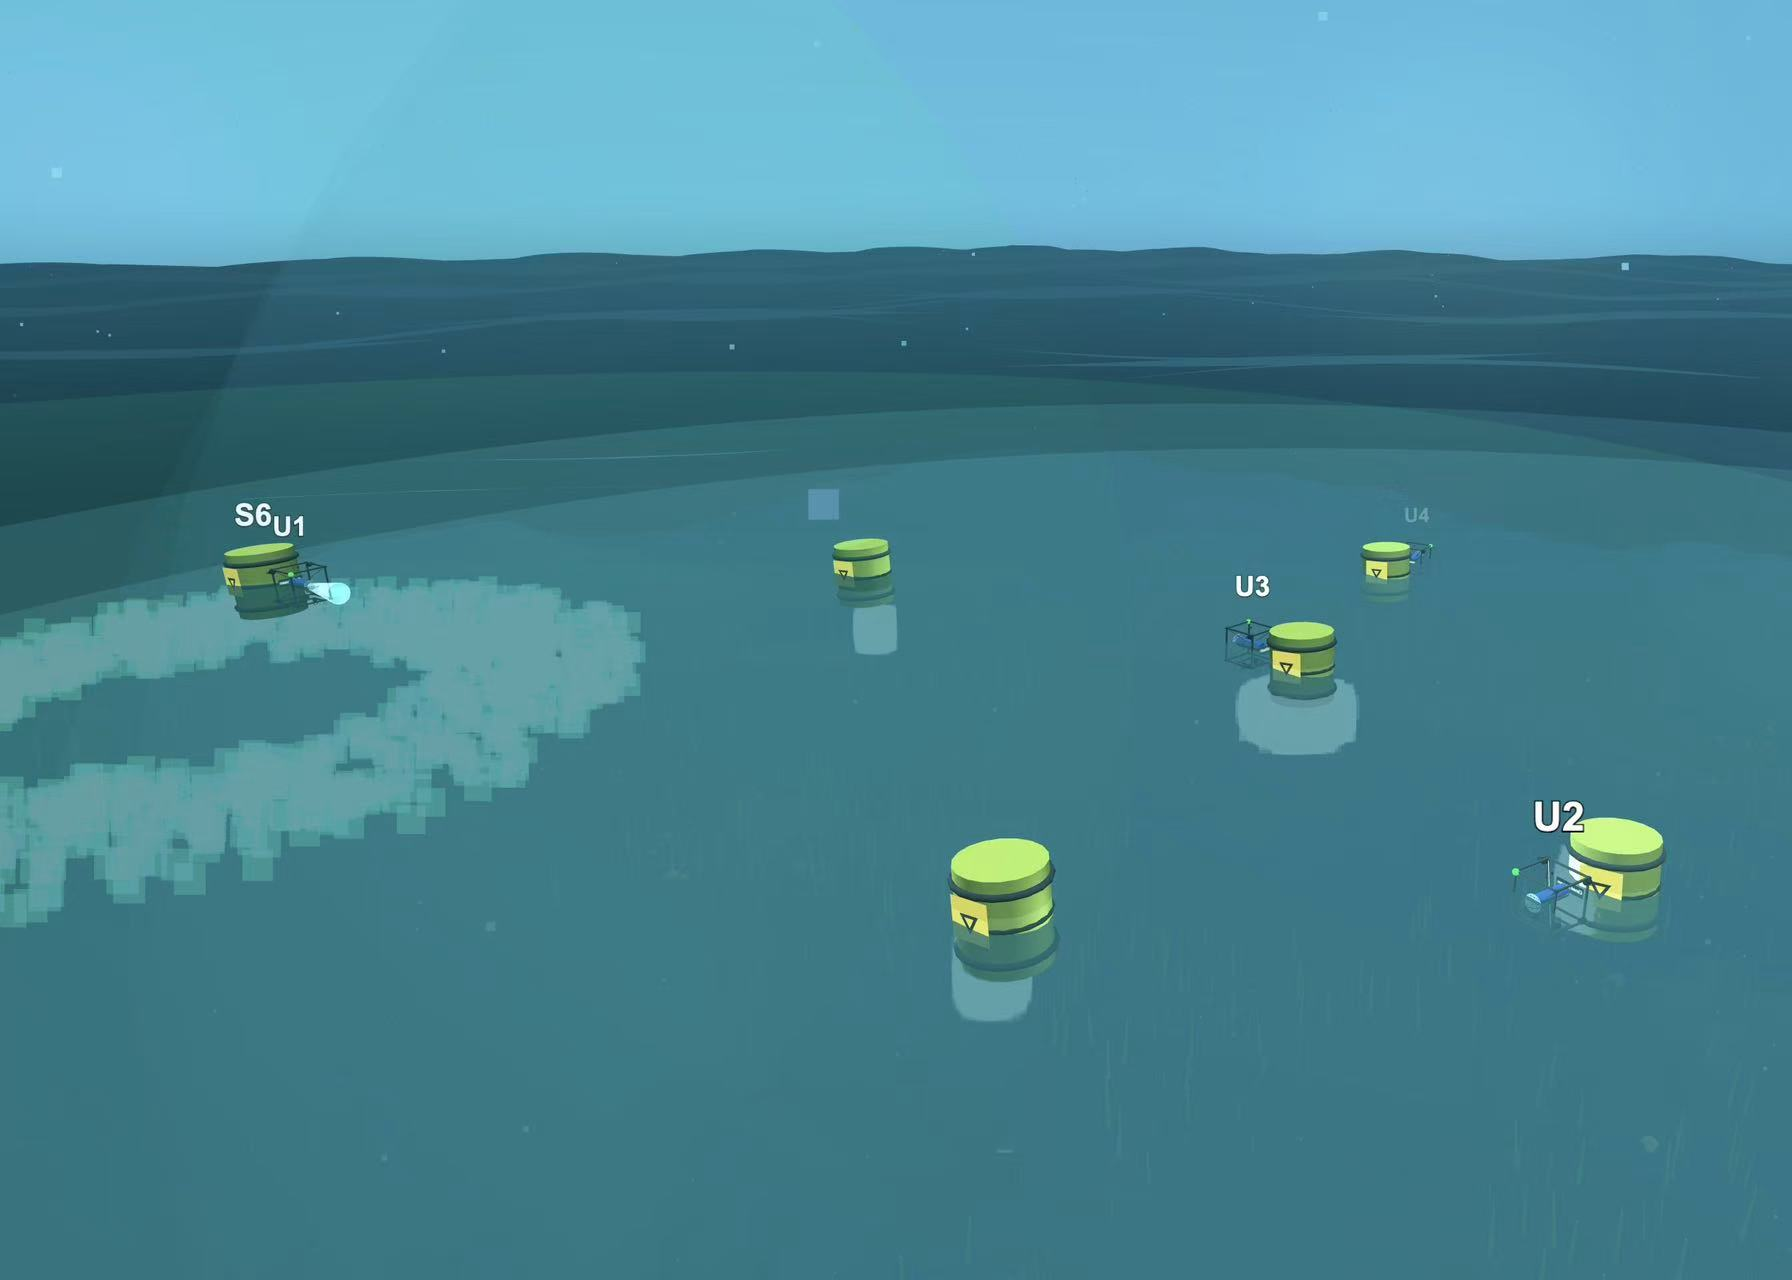
\includegraphics[width=0.48\linewidth]{figures/task1_ui_off.png}}
 \hfill
 \subfloat[UPL: Underwater Pollution Lift (5 UUVs)]{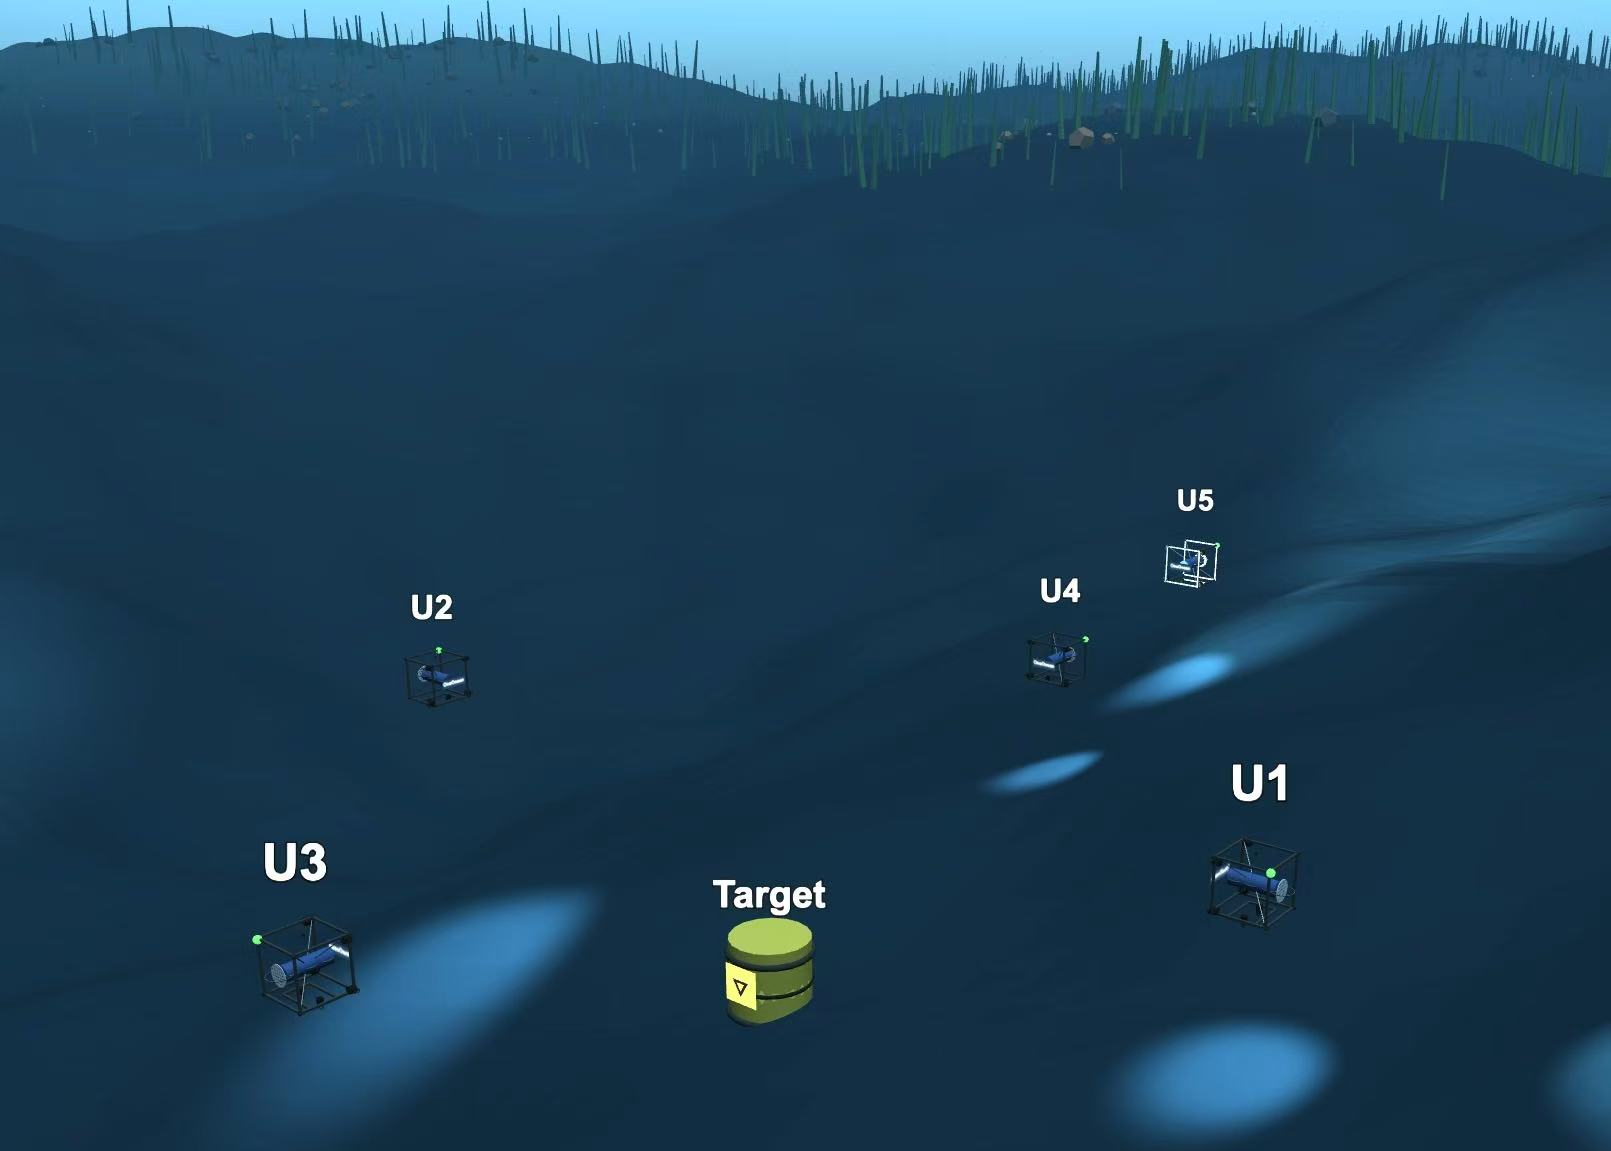
\includegraphics[width=0.48\linewidth]{figures/task2_ui_off.png}}\\
 \subfloat[AS: Area Scan over terrain]{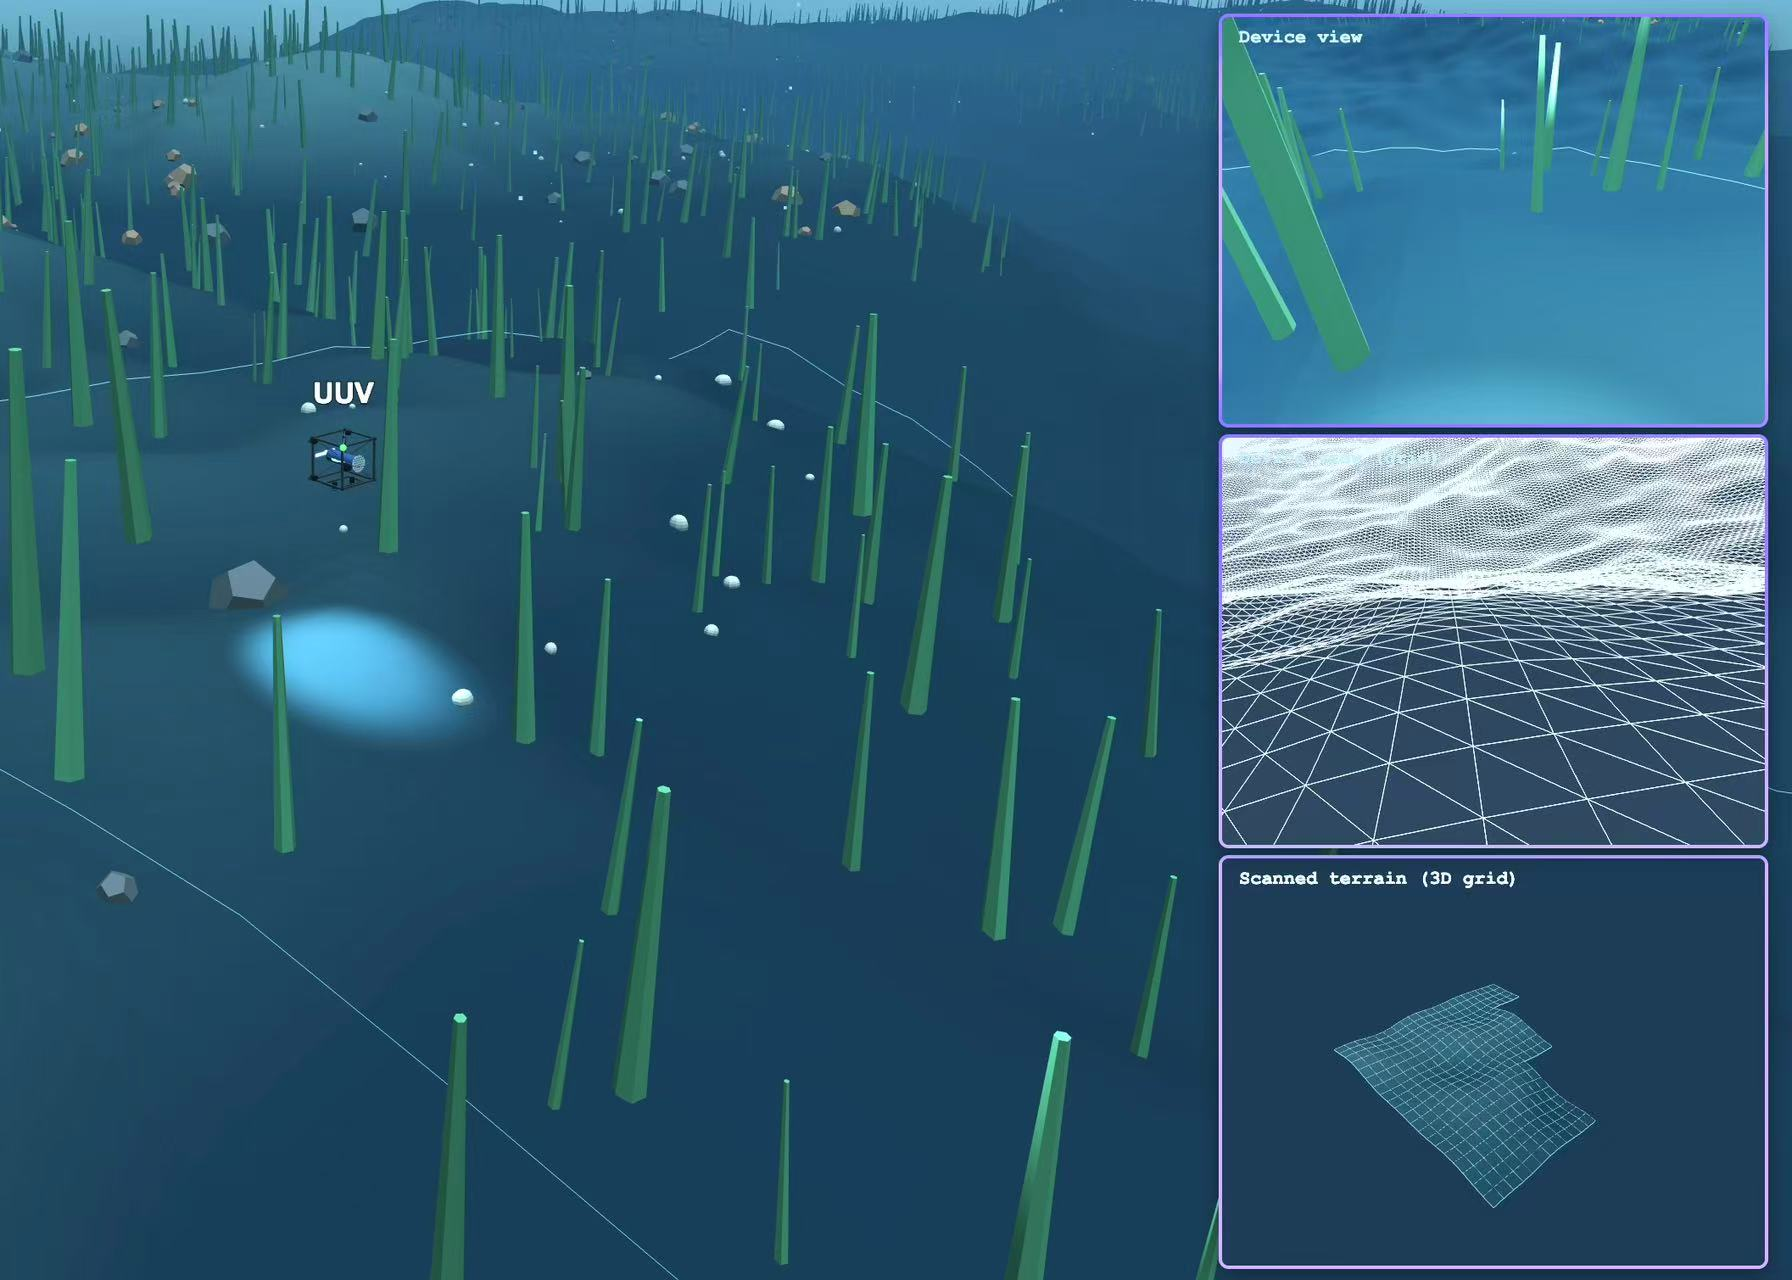
\includegraphics[width=0.48\linewidth]{figures/task4_ui_off.png}}
 \hfill
 \subfloat[FH: Fish Protection / Herding (8 UUVs)]{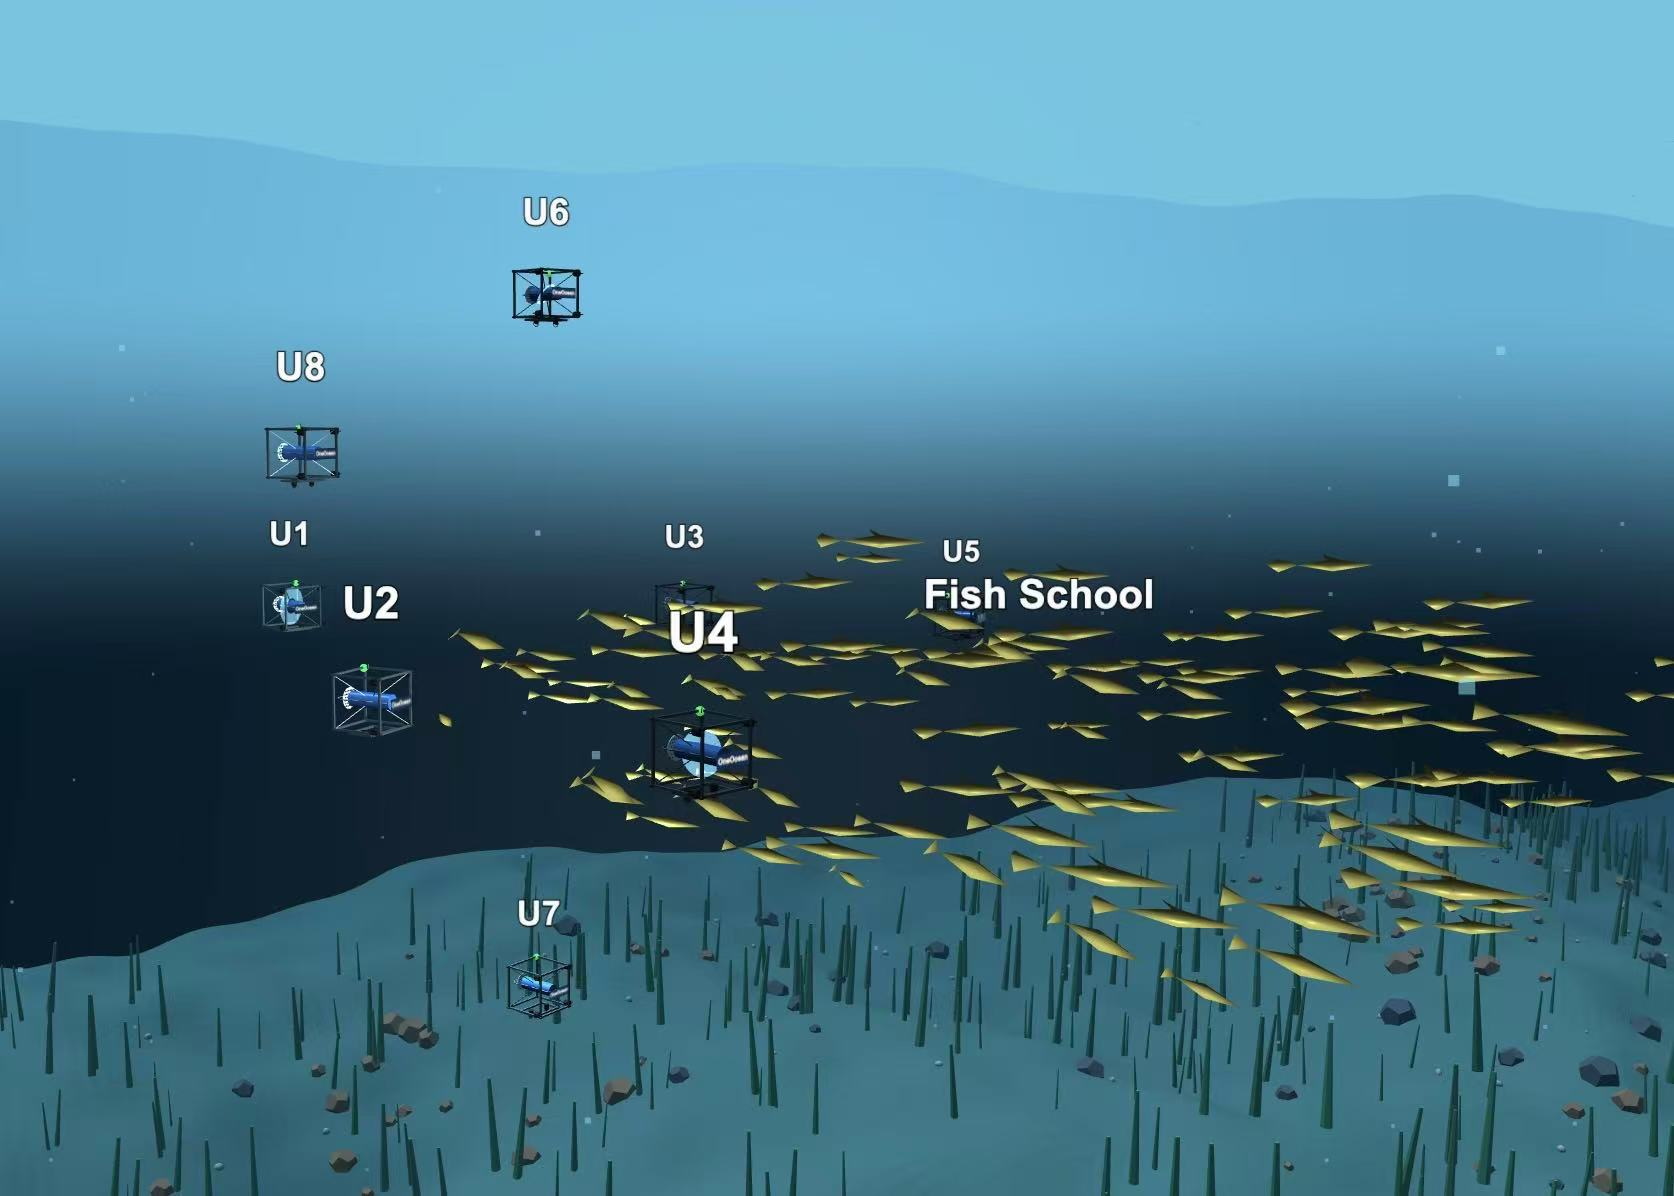
\includegraphics[width=0.48\linewidth]{figures/task3_ui_off.png}}
 \caption{Surface Pollution Cleanup, Underwater Pollution Lift, Area Scan, and Fish Protection / Herding in the core backend.}
 \label{fig:core_ui_off_panel}
\end{figure}
}


\revise{
\begin{table}[t]
\centering
\scriptsize
\setlength{\tabcolsep}{1.2pt}
\renewcommand{\arraystretch}{1.10}
\begin{tabularx}{\columnwidth}{@{}>{\raggedright\arraybackslash}p{0.26\columnwidth}*{7}{Y}@{}}
\toprule
\textbf{Method} & \makecell{\textbf{Avg.}\\\textbf{SR(\%)}} & \makecell{\textbf{Calls}} & \makecell{\textbf{Lat.}\\\textbf{(s)}} & \makecell{\textbf{ms per}\\\textbf{call}} & \makecell{\textbf{Prompt}\\\textbf{tok.}} & \makecell{\textbf{Output}\\\textbf{tok.}} & \makecell{\textbf{Total}\\\textbf{tok.}} \\
\midrule
\rowcolor{oursbg}
LLM-Qwen2.5-7B & \best{65.0} & 6.48 & 14.21 & 2222.1 & 3932 & 4084 & 8016 \\
LLM-Qwen2-7B & 53.3 & \best{4.71} & 11.24 & 2440.3 & 2877 & 2996 & 5873 \\
LLM-Mistral-7B & 53.3 & 6.05 & 31.38 & 4942.5 & 3762 & 4128 & 7890 \\
LLM-ChatGLM3-6B & 53.3 & 5.38 & \best{7.91} & \best{1393.6} & 3414 & \best{411} & \best{3825} \\
\rowcolor{oursbg}
Heuristic & 55.0 & \best{0.00} & \best{0.00} & \best{0.0} & \best{0} & \best{0} & \best{0} \\
LLM-Llama3-8B & 45.0 & 6.71 & 13.94 & 2117.5 & 3072 & 3218 & 6292 \\
LLM-Llama2-7B & 33.3 & 6.59 & 49.42 & 7401.8 & 4219 & 4851 & 9071 \\
BC & 21.7 & \best{0.00} & \best{0.00} & \best{0.0} & \best{0} & \best{0} & \best{0} \\
\bottomrule
\end{tabularx}
\caption{Core-benchmark planning-suite cost metrics at Tier 2 with doubled currents: uncached local-inference calls, latency, and token usage, reported alongside average success over 20 episodes per task.}
\label{tab:planning_suite_cost_t2}
\end{table}
}

\revise{Across ten tasks, heuristic success decreases from 84.6\% at Tier 2 to 29.0\% at Tier 3, while BC decreases from 58.6\% to 6.0\% (Table~\ref{tab:headline_macro_keymetrics}). Table~\ref{tab:per_task_sr_t2_t3} reports the task-level changes, including gaps in Station Keeping, Route Following, Surface Pollution Cleanup, and Pipeline Inspection. Figure~\ref{fig:core_ui_off_panel} shows four tasks from the suite.}

\revise{Figure~\ref{fig:difficulty_ladder_dualpanel} compares success across all three tiers for a five-task subset.}

\revise{
\begin{figure*}[t]
 \centering
 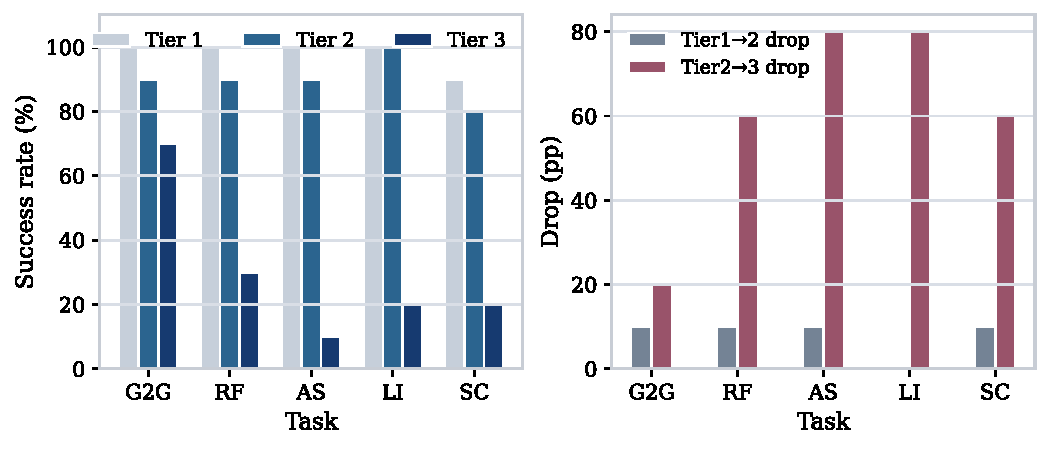
\includegraphics[width=0.98\textwidth]{figures/difficulty_ladder_dualpanel.pdf}
 \caption{Success rates across difficulty tiers for a five-task subset. Left: success rate at Tiers~1--3. Right: success-rate drops from Tier~1$\rightarrow$2 and Tier~2$\rightarrow$3.}
 \label{fig:difficulty_ladder_dualpanel}
\end{figure*}
}

\revise{Heuristic control has higher macro success at both tiers. BC performs well on \emph{Underwater Pollution Lift (UPL)} and \emph{Fish Protection / Herding (FH)} at Tier 2, but declines on tasks requiring persistent disturbance rejection or coordinated geometry. In Surface Pollution Cleanup, larger teams improve success and source completion while increasing collision exposure (Figure~\ref{fig:cleanup_scaling_dualpanel}). The action-energy proxy varies non-monotonically with team size.}

\paragraph{Planning-sensitive tasks.}

\revise{We compare deterministic heuristic control, BC, and local LLM planners on Surface Pollution Cleanup (SPC), Area Scan (AS), and Pipeline Inspection (PI). Each LLM proposes assignments or waypoints at a fixed stride; a deterministic controller executes them with shared safety checks.}

\revise{In the 40-episode-per-task study, heuristic control has the highest average success (Table~\ref{tab:planning_suite_perf_t2}). ChatGLM3-6B matches its cleanup rate and achieves the highest scan coverage. In the separate 20-episode-per-task cost study, Qwen2.5-7B has the highest average success, and ChatGLM3-6B has the lowest LLM inference latency (Table~\ref{tab:planning_suite_cost_t2}).}

\revise{In the three-seed planning diagnostic, valid plans can revisit covered cells or miss leaks, while invalid responses invoke the deterministic task allocator. We report executed command effort through $E$ and inference cost through latency and token counts. Appendix Sec.~\ref{supp-app:core_diagnostics} reports task-level and model-level validity, fallback, completion, token, and latency values.}

\revise{
\begin{figure*}[t]
 \centering
 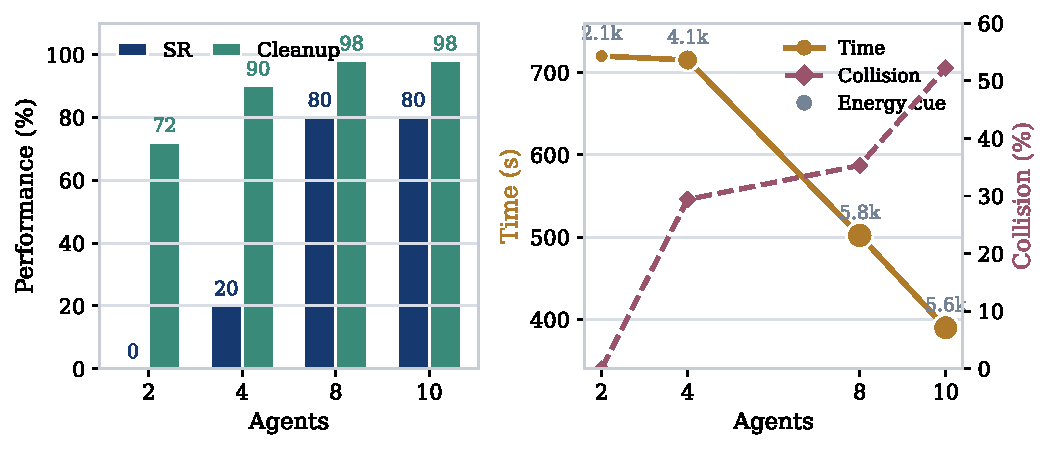
\includegraphics[width=0.98\textwidth]{figures/cleanup_scaling_dualpanel.pdf}
 \caption{Surface-cleanup scaling at Tier~2. Left: success rate and cleanup rate as the number of vehicles increases. Right: completion time and near-collision ratio, with per-point annotations showing the energy proxy in thousands.}
 \label{fig:cleanup_scaling_dualpanel}
\end{figure*}
}

\subsection{External underwater-scene backend}

\revise{
\begin{figure}[ht]
 \centering
 \subfloat[Surface pollution containment and cleanup in a packaged ocean scene.]{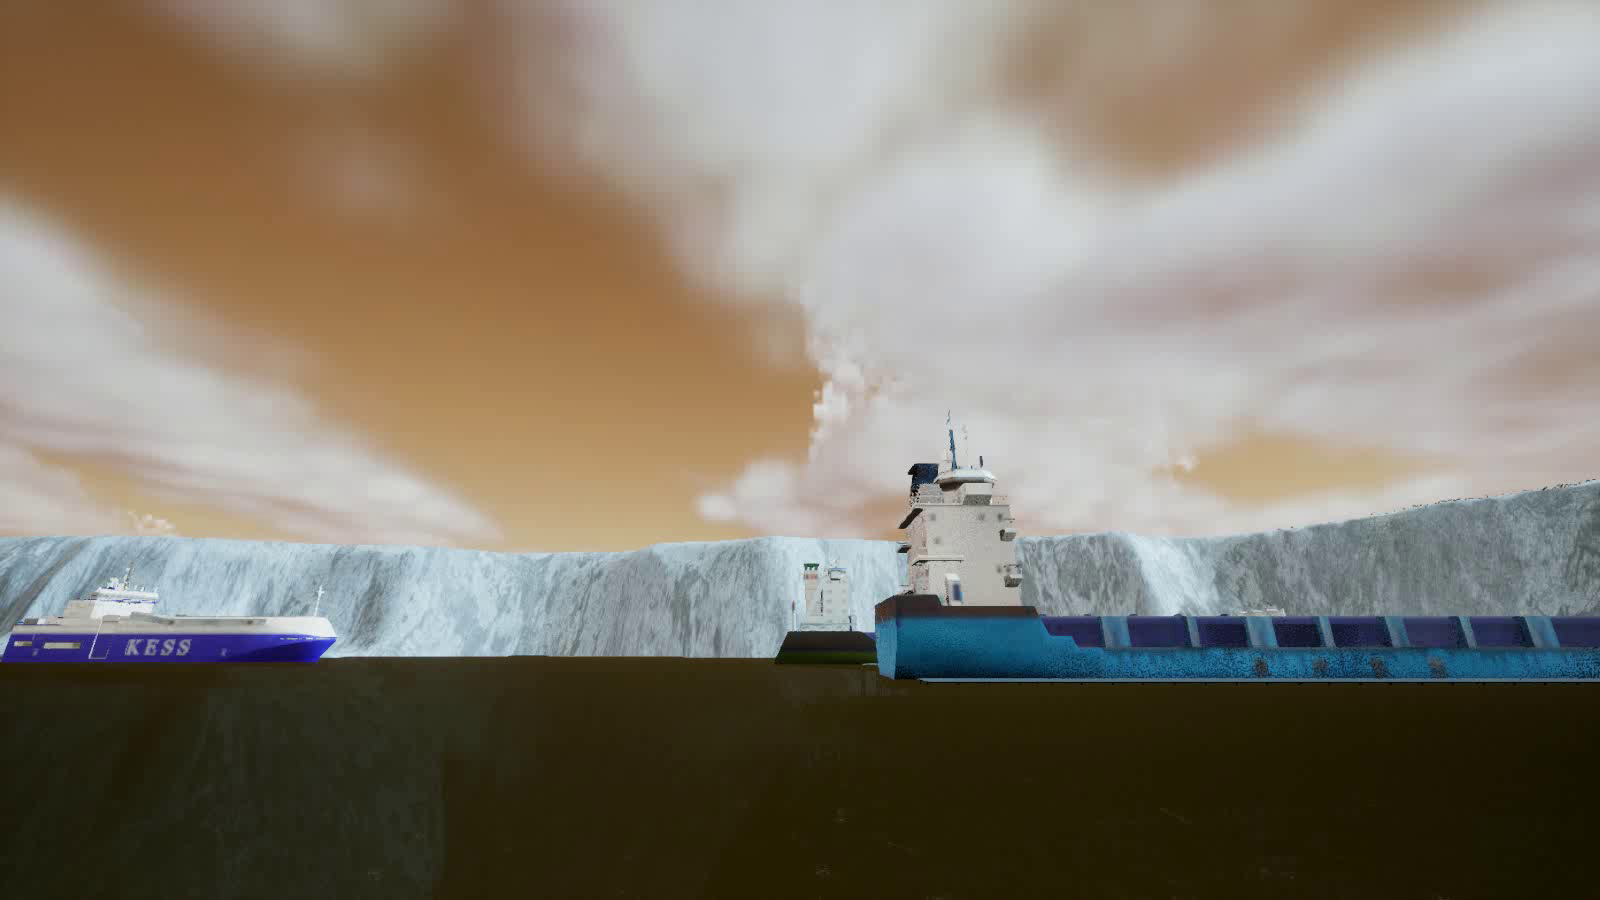
\includegraphics[width=0.48\linewidth]{figures/h3_oceangym_image1_containment.jpg}}
 \hfill
 \subfloat[Multi-agent scene-backed deployment.]{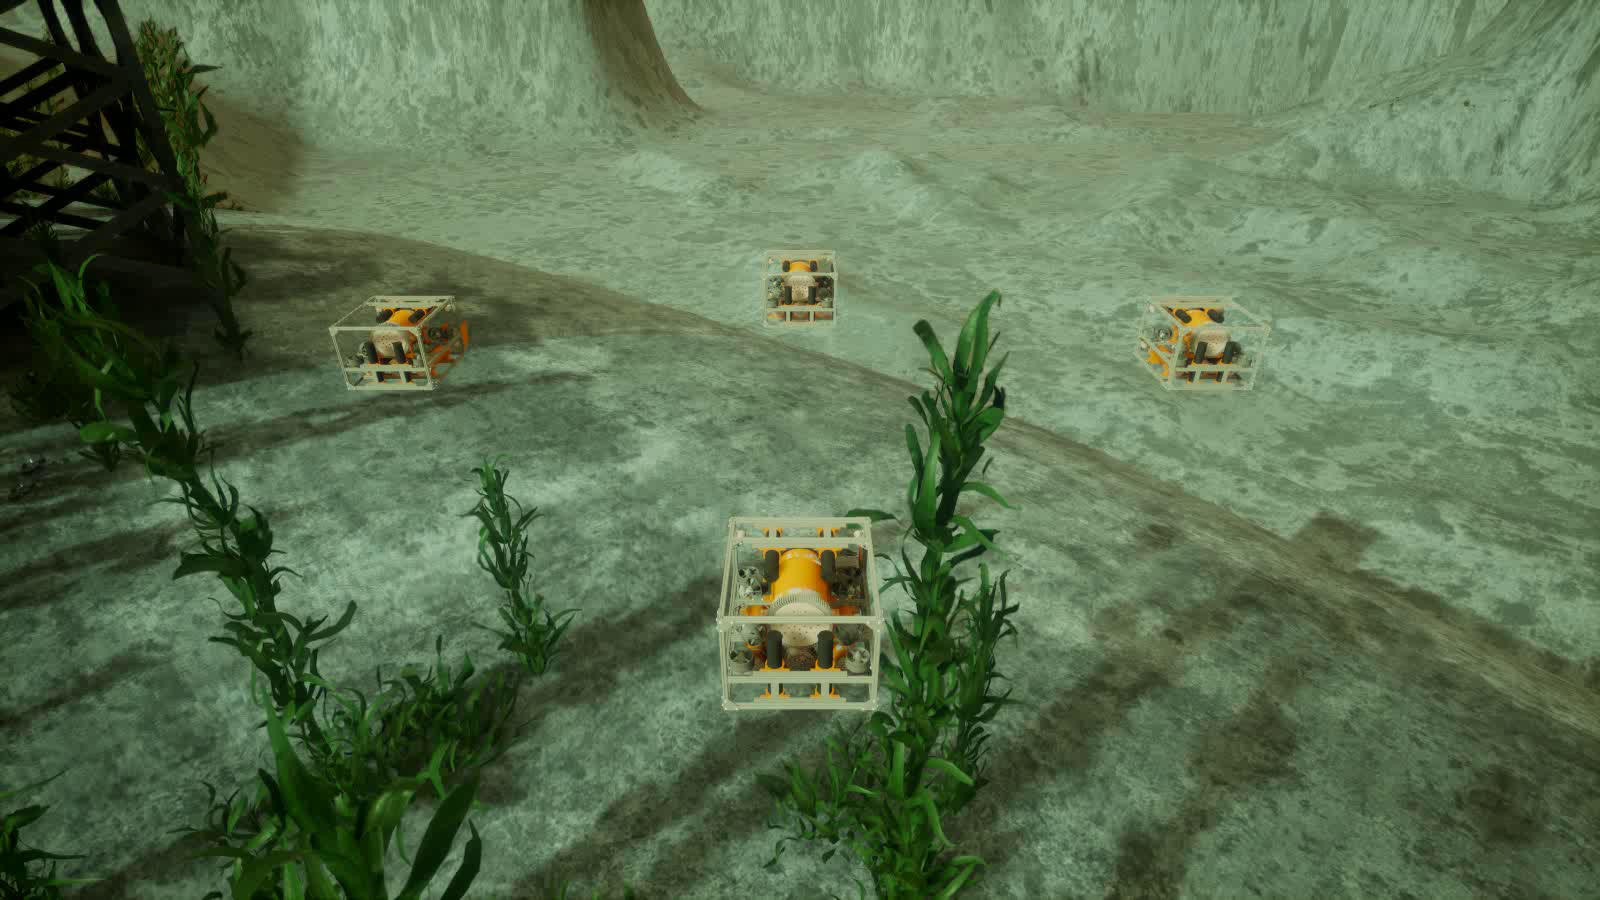
\includegraphics[width=0.48\linewidth]{figures/h3_oceangym_image2_formation.jpg}}
 \caption{Task demonstrations in packaged underwater scenes using currents exported from the OneOcean dataset.}
 \label{fig:extscene_keyframes}
\end{figure}
}

\revise{Route-following performance varies across four underwater scenes (Table~\ref{tab:h3_route_generalization}), while Figure~\ref{fig:extscene_keyframes} shows pollution-response and multi-agent demonstrations. The scene backend introduces scene geometry and applies currents through a one-way disturbance interface. A separate diagnostic found lower localization error with OCPNet-3D under both tested current settings, with aggregate success matching or exceeding the analytic probe. Appendix Sec.~\ref{supp-app:external_diagnostics} provides the values and episode budgets.}

\revise{
\begin{table}[t]
\centering
\scriptsize
\setlength{\tabcolsep}{1.2pt}
\renewcommand{\arraystretch}{1.12}
\begin{tabularx}{\columnwidth}{@{}>{\raggedright\arraybackslash}p{0.25\columnwidth}*{6}{Y}@{}}
\toprule
\multirow{2}{*}{\textbf{Scene}} & \multicolumn{3}{c}{\textbf{Tier 2}} & \multicolumn{3}{c}{\textbf{Tier 3}} \\
\cmidrule(lr){2-4}\cmidrule(lr){5-7}
 & \makecell{SR\\(\%)} & \makecell{WP} & \makecell{CTE\\(m)} & \makecell{SR\\(\%)} & \makecell{WP} & \makecell{CTE\\(m)} \\
\midrule
Dam & 0.0 & 1.0 & 3.06 & 0.0 & 0.0 & \best{0.87} \\
OpenWater & 20.0 & 3.1 & 2.50 & 0.0 & 0.0 & 1.91 \\
PierHarbor & 56.7 & 3.5 & \best{2.22} & 0.0 & 2.0 & 1.41 \\
SimpleUnderw. & \best{100.0} & \best{4.0} & 3.04 & \best{96.7} & \best{3.0} & 2.16 \\
\rowcolor{scenarioGray}
Mean over scenes & 44.2 & 2.92 & 2.70 & 24.2 & 1.25 & 1.59 \\
\bottomrule
\end{tabularx}
\caption{Route-following across four underwater scenes, with 30 episodes per difficulty in each scene. WP denotes the mean number of reached waypoints; CTE denotes Cross-Track Error.}
\label{tab:h3_route_generalization}
\end{table}
}
